\documentclass[11pt,a4paper,twoside]{article}
\usepackage[left=20mm, right=20mm, top=20mm, bottom=20mm]{geometry}
\usepackage{setspace}
\onehalfspacing
\usepackage[T1]{fontenc}
\usepackage[croatian]{babel}

\usepackage[dvipsnames]{xcolor}
\usepackage[most]{tcolorbox}
\definecolor{blue1}{HTML}{DEE3E9}
\definecolor{blue2}{HTML}{F9F9F9}
\definecolor{blue3}{HTML}{9EADC0}

\definecolor{solarized@red}{HTML}{bc658d}
\definecolor{solarized@blue}{HTML}{4677CB}
\definecolor{solarized@green}{HTML}{82c4c3}
\definecolor{solarized@orange}{HTML}{f9d89c}
\definecolor{solarized@background}{HTML}{fbfbfb}

\newenvironment{infoBox}
{
	\begin{tcolorbox}[colback=solarized@background,colframe=solarized@green,enlarge top by=6pt, enlarge bottom by=6pt, title=Informacija]
	}{
	\end{tcolorbox}	
}

\newenvironment{warningBox}
{
	\begin{tcolorbox}[colback=solarized@background,colframe=solarized@orange,enlarge top by=6pt, enlarge bottom by=6pt, title=Upozorenje]
	}{
	\end{tcolorbox}
}

\newenvironment{errorBox}
{
	\begin{tcolorbox}[colback=solarized@background,colframe=solarized@red,enlarge top by=6pt, enlarge bottom by=6pt, title=Mogući problem]
	}{	
	\end{tcolorbox}
}

\newenvironment{comicBox}
{
	\begin{tcolorbox}[colback=solarized@background,colframe=solarized@blue,enlarge top by=6pt, enlarge bottom by=6pt, title=Comic]
	}{	
	\end{tcolorbox}
}

\usepackage{listings}

\lstset
{
	basicstyle=\tiny,
	numbers=left,
	numbersep=5pt,
	numberstyle=\tiny\color{gray},
	showspaces=false,
	tabsize=2,
	columns=fullflexible,
	frame=tb,
	breaklines=true,
	postbreak=\mbox{\textcolor{red}{$\hookrightarrow$}\space},
	xleftmargin=17pt,
	xrightmargin=6pt,
	framexleftmargin=17pt,
	framexrightmargin=5pt,
	framexbottommargin=4pt,
    showstringspaces=false,
}

\lstdefinelanguage{XML}
{
	morestring=[b]",
	morestring=[s]{>}{<},
	morecomment=[s]{<?}{?>},
	stringstyle=\color{black},
	identifierstyle=\color{black},
	keywordstyle=\color{cyan},
	morekeywords={xmlns,version,type,ma-id}% list your attributes here
}

\lstdefinelanguage{Kotlin}
{
	comment=[l]{//},
	commentstyle={\color{gray}\ttfamily},
	emph={filter, first, firstOrNull, forEach, lazy, map, mapNotNull, println},
	emphstyle={\color{OrangeRed}},
	identifierstyle=\color{black},
	keywords={!in, !is, abstract, actual, annotation, as, as?, break, by, catch, class, companion, const, constructor, continue, crossinline, data, delegate, do, dynamic, else, enum, expect, external, false, field, file, final, finally, for, fun, get, if, import, in, infix, init, inline, inner, interface, internal, is, lateinit, noinline, null, object, open, operator, out, override, package, param, private, property, protected, public, receiveris, reified, return, return@, sealed, set, setparam, super, suspend, tailrec, this, throw, true, try, typealias, typeof, val, var, vararg, when, where, while},
	keywordstyle={\color{NavyBlue}\bfseries},
	morecomment=[s]{/*}{*/},
	morestring=[b]",
	morestring=[s]{"""*}{*"""},
	ndkeywords={@Deprecated, @JvmField, @JvmName, @JvmOverloads, @JvmStatic, @JvmSynthetic, Array, Byte, Double, Float, Int, Integer, Iterable, Long, Runnable, Short, String, Any, Unit, Nothing},
	ndkeywordstyle={\color{BurntOrange}\bfseries},
	sensitive=true,
	stringstyle={\color{ForestGreen}\ttfamily},
} 

% Handling figures:
\usepackage{graphicx}
\graphicspath{{../figures/}}

\begin{document}
	
\section{Uvod}

	Razvoj mobilnih aplikacija jedna je od radionica u sklopu projekta Studentsko poduzetništvo - 404 koji se izvodi 2023. u suradnji Fakulteta elektrotehnike, računarstva i informacijskih tehnologija Osijek (FERIT), Fakulteta primijenjene matematike i informatike u Osijeku (MATHOS) te Ekonomskog fakulteta u Osijeku (EFOS). Cilj radionice jest pokazati učenicima osnovne koncepte razvoja mobilnih aplikacija s fokusom na platformu Android te ih potaknuti na samostalno učenje i istraživanje.
	
	Ovaj minijaturni priručnik prati aktivnosti radionice gdje će se kroz kreiranje nove Android aplikacije učenici upoznati s osnovnim pojmovima kao što su izgradnja korisničkog sučelja, povezivanje programskog koda i elemenata korisničkog sučelja, ali i sa složenijim elementima aplikacija poput uporabe senzora ili prikaza podataka dostupnih na Internetu. Aplikacija koja će biti izrađena sastoji se od tri zasebna ekrana, ekrana za inspiraciju koji će poslužiti za prolazak kroz osnove kreiranja korisničkog sučelja, ekrana za igru koji će poslužiti za upoznavanje sa senzorima te ekrana za šalu koji će poslužiti za dohvaćanje podataka s interneta i njihov prikaz. Svijet razvoja mobilnih aplikacija puno je širi od sadržaja koji pokriva radionica pa će u posljednjem poglavlju biti prikazane poveznice na vanjske resurse koje je moguće koristiti za samostalan rad i učenje. Za sve naknadne informacije i pitanja, slobodno se javite putem e-maila na bruno.zoric@ferit.hr.
	
	\begin{infoBox}		
		
	\end{infoBox}
	
\section{Instalacija alata}

\begin{figure}[!h]
	\centering
	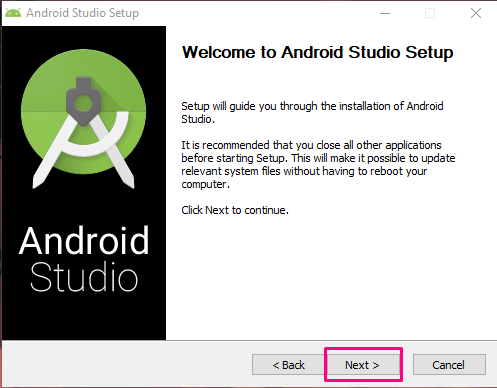
\includegraphics{install_01.png}
	\caption{Instalacija Android Studija - 1. korak}
	\label{fig:install_01}	
\end{figure}

\begin{figure}[!h]
	\centering
	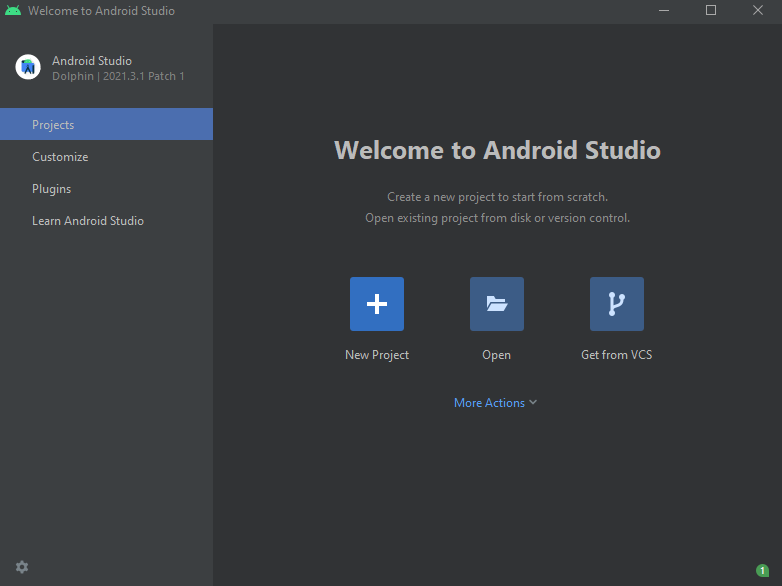
\includegraphics[width=\textwidth]{install_02.png}
	\caption{Instalacija Android Studija - 2. korak}
	\label{fig:install_02}	
\end{figure}

\begin{figure}[!h]
	\centering
	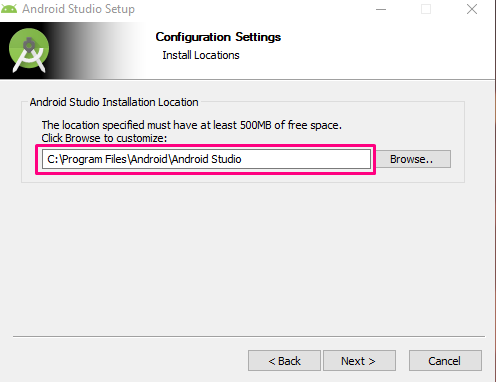
\includegraphics{install_03.png}
	\caption{Instalacija Android Studija - 3. korak}
	\label{fig:install_03}	
\end{figure}

\begin{figure}[!h]
	\centering
	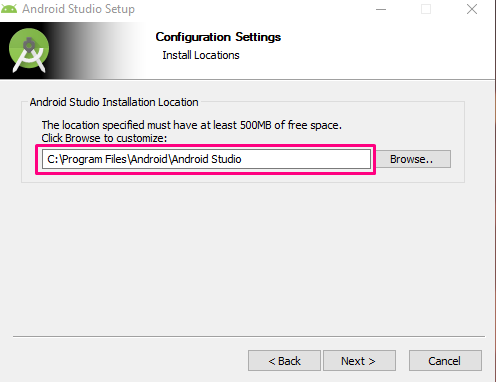
\includegraphics{install_04.png}
	\caption{Instalacija Android Studija - 3. korak}
	\label{fig:install_03}	
\end{figure}

\begin{figure}[!h]
	\centering
	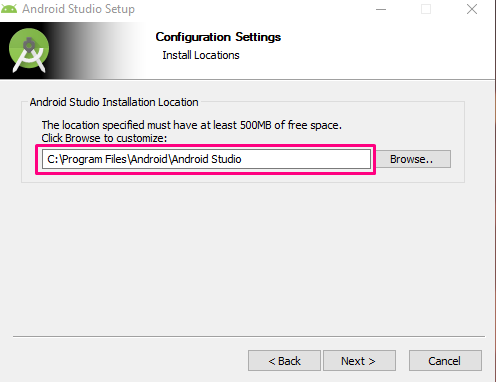
\includegraphics{install_04.png}
	\caption{Instalacija Android Studija - 4. korak}
	\label{fig:install_04}	
\end{figure}

\begin{figure}[!h]
	\centering
	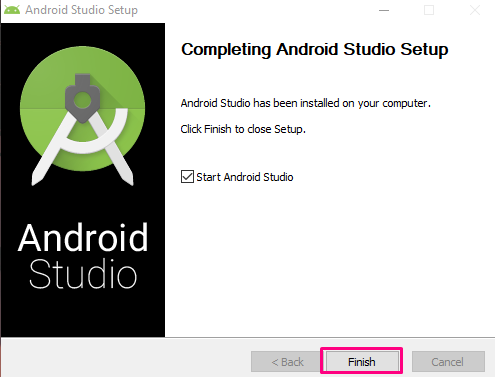
\includegraphics{install_05.png}
	\caption{Instalacija Android Studija - 5. korak}
	\label{fig:install_05}	
\end{figure}

\begin{figure}[!h]
	\centering
	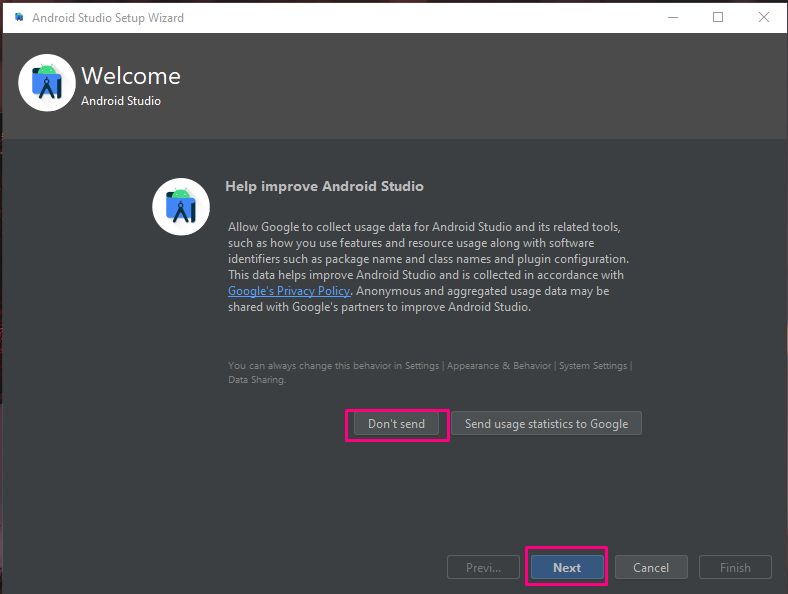
\includegraphics{install_06.png}
	\caption{Instalacija Android Studija - 6. korak}
	\label{fig:install_06}	
\end{figure}

\begin{figure}[!h]
	\centering
	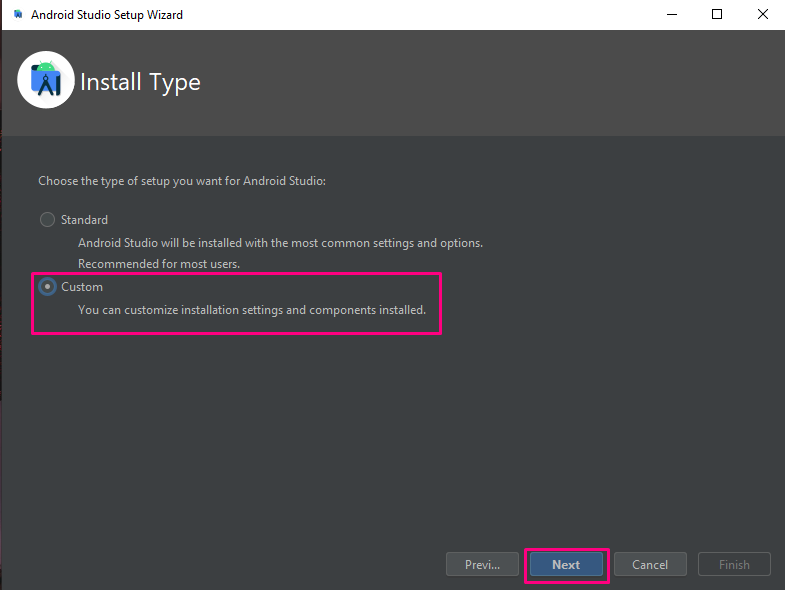
\includegraphics[width=\textwidth]{install_07.png}
	\caption{Instalacija Android Studija - 7. korak}
	\label{fig:install_07}	
\end{figure}

\begin{figure}[!h]
	\centering
	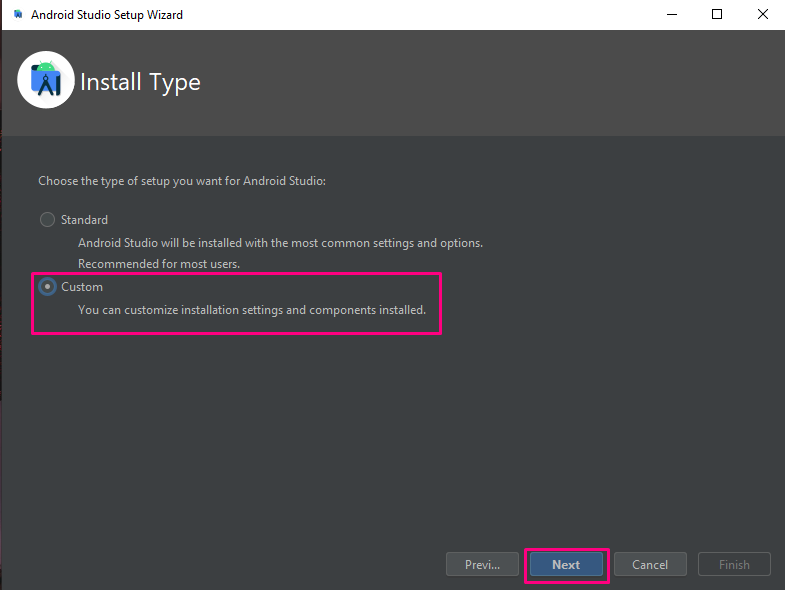
\includegraphics[width=\textwidth]{install_08.png}
	\caption{Instalacija Android Studija - 8. korak}
	\label{fig:install_08}	
\end{figure}

\begin{figure}[!h]
	\centering
	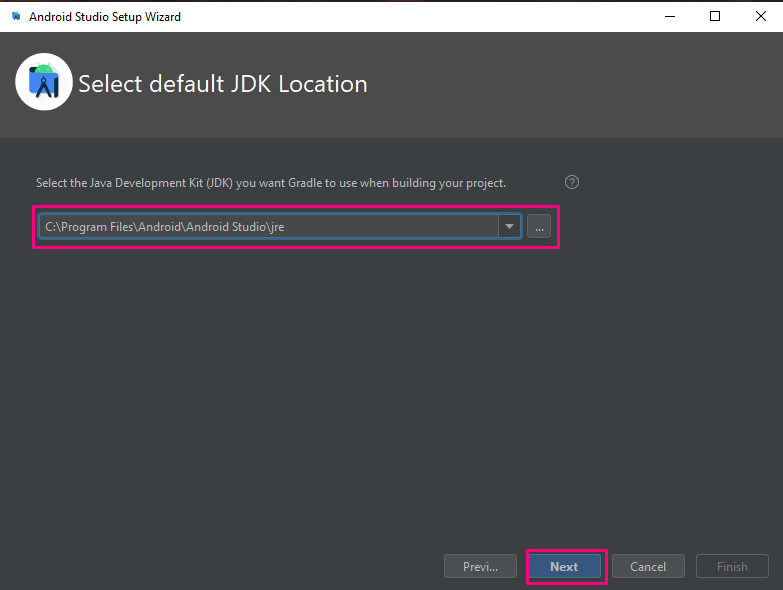
\includegraphics[width=\textwidth]{install_09.png}
	\caption{Instalacija Android Studija - 9. korak}
	\label{fig:install_09}	
\end{figure}

\begin{figure}[!h]
	\centering
	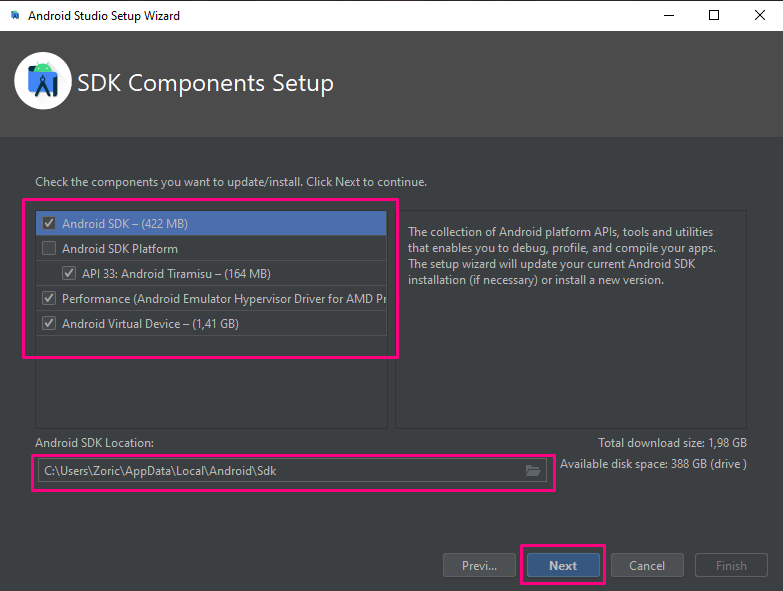
\includegraphics[width=\textwidth]{install_10.png}
	\caption{Instalacija Android Studija - 10. korak}
	\label{fig:install_10}	
\end{figure}

\begin{figure}[!h]
	\centering
	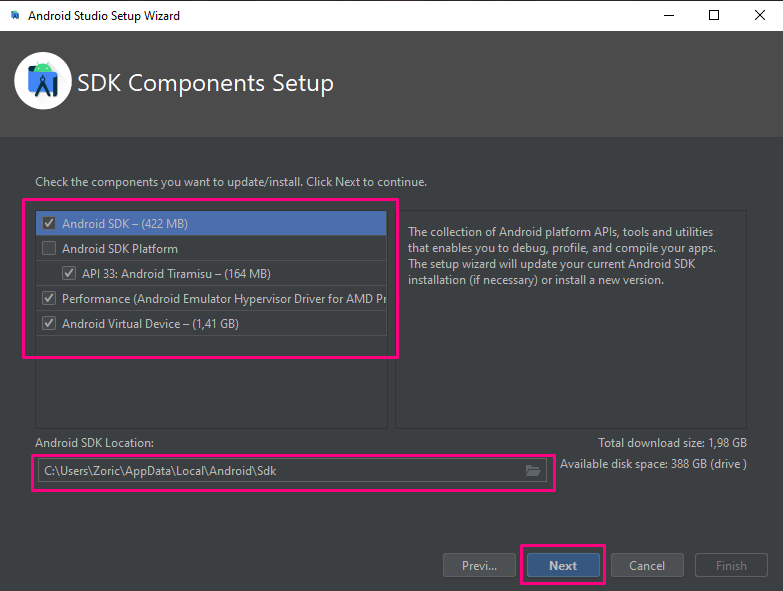
\includegraphics[width=\textwidth]{install_11.png}
	\caption{Instalacija Android Studija - 11. korak}
	\label{fig:install_11}	
\end{figure}

\begin{figure}[!h]
	\centering
	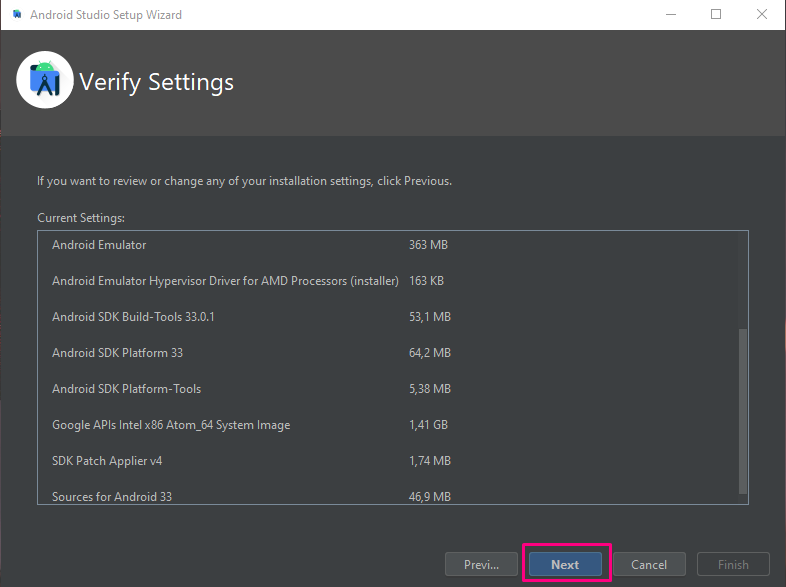
\includegraphics[width=\textwidth]{install_12.png}
	\caption{Instalacija Android Studija - 12. korak}
	\label{fig:install_12}	
\end{figure}

\begin{figure}[!h]
	\centering
	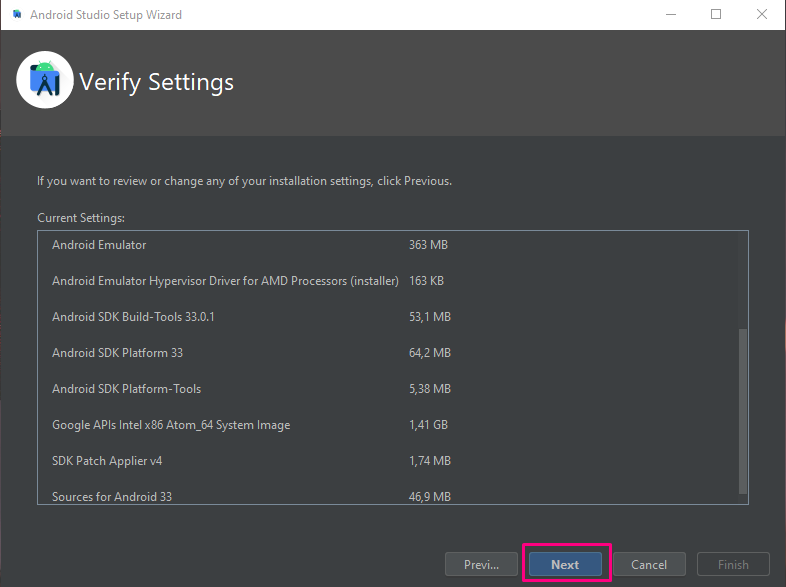
\includegraphics[width=\textwidth]{install_13.png}
	\caption{Instalacija Android Studija - 13. korak}
	\label{fig:install_13}	
\end{figure}

\begin{figure}[!h]
	\centering
	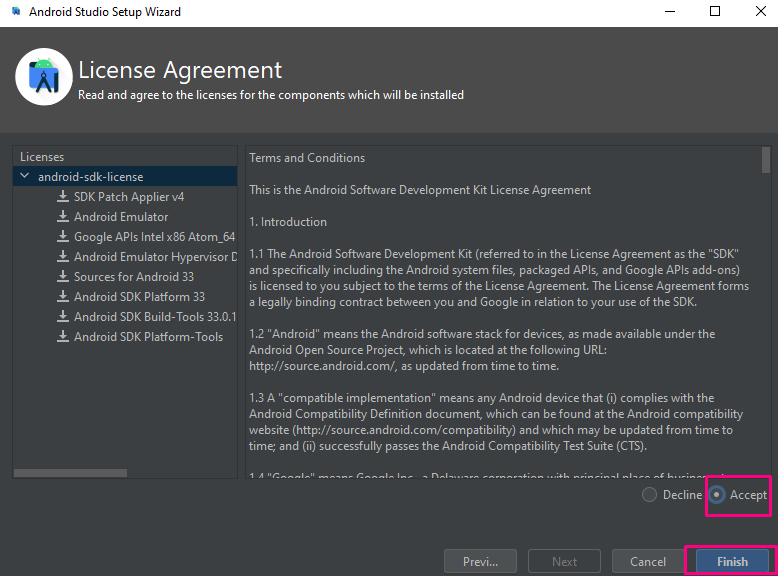
\includegraphics[width=\textwidth]{install_14.png}
	\caption{Instalacija Android Studija - 14. korak}
	\label{fig:install_14}	
\end{figure}

\begin{figure}[!h]
	\centering
	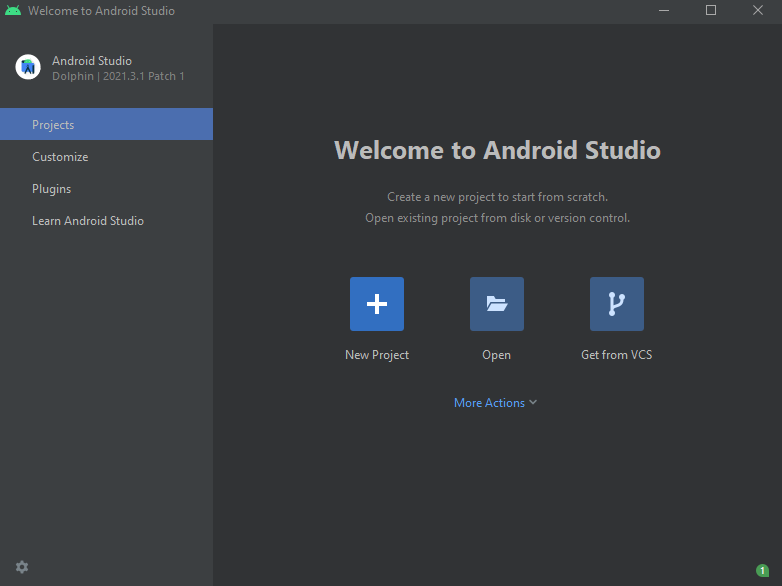
\includegraphics[width=\textwidth]{install_15.png}
	\caption{Instalacija Android Studija - 15. korak}
	\label{fig:install_15}	
\end{figure}

\section{Kreiranje projekta}

\begin{figure}[!h]
	\centering
	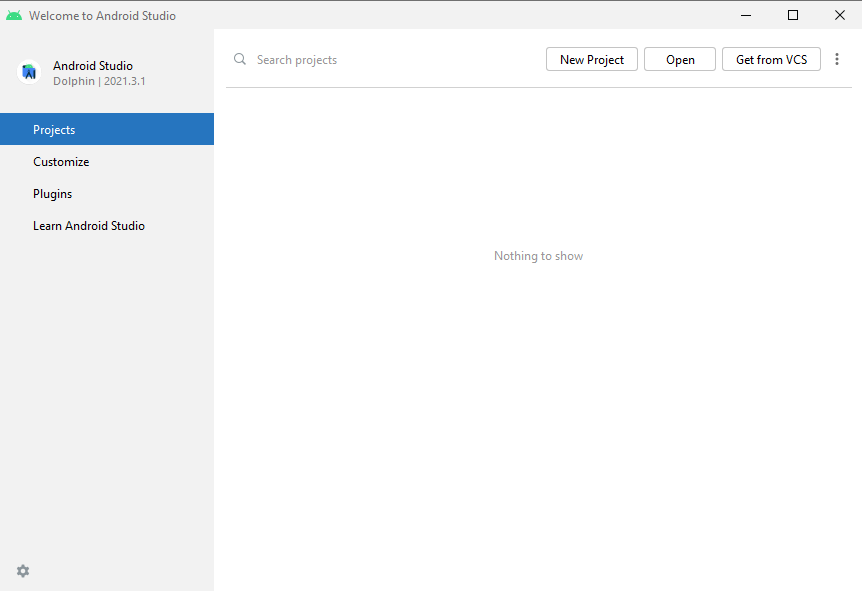
\includegraphics[width=\textwidth]{new_project_01.png}
	\caption{Kreiranje novog projekta - 1. korak}
	\label{fig:new_project_01}	
\end{figure}

\begin{figure}[!h]
	\centering
	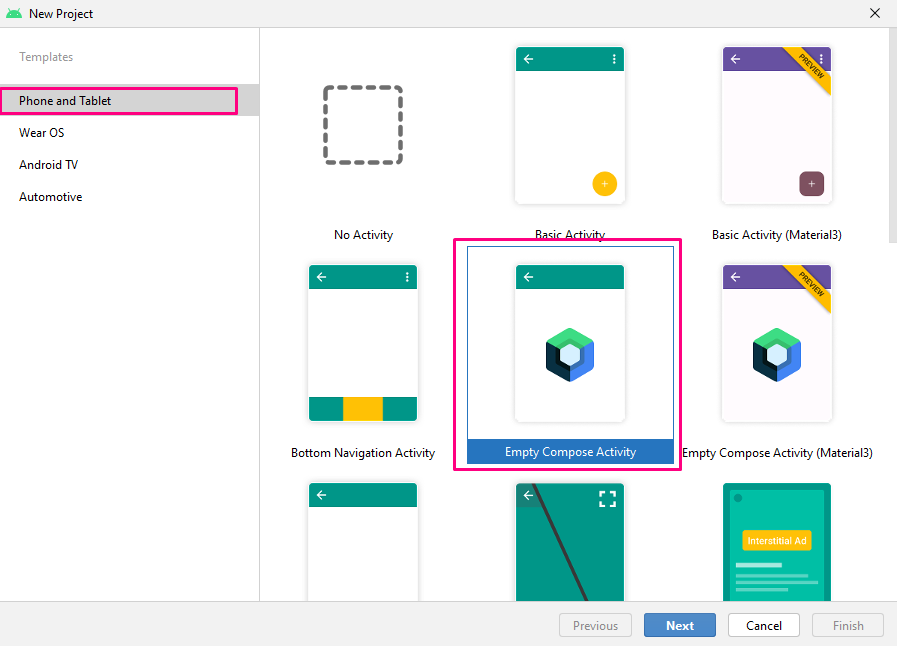
\includegraphics[width=\textwidth]{new_project_02.png}
	\caption{Kreiranje novog projekta - 2. korak}
	\label{fig:new_project_02}	
\end{figure}

\begin{figure}[!h]
	\centering
	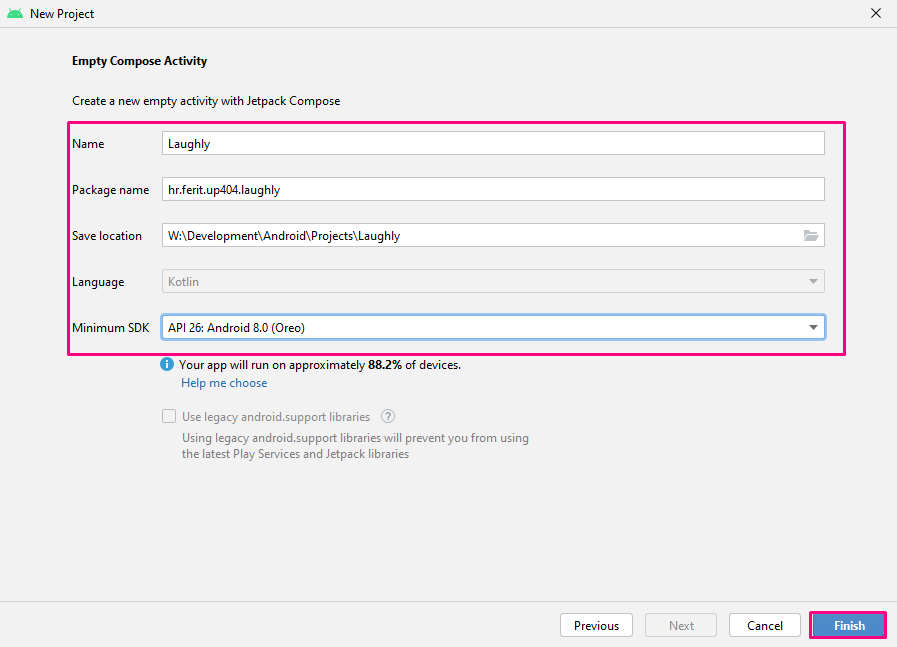
\includegraphics[width=\textwidth]{new_project_03.png}
	\caption{Kreiranje novog projekta - 3. korak}
	\label{fig:new_project_03}	
\end{figure}

\begin{figure}[!h]
	\centering
	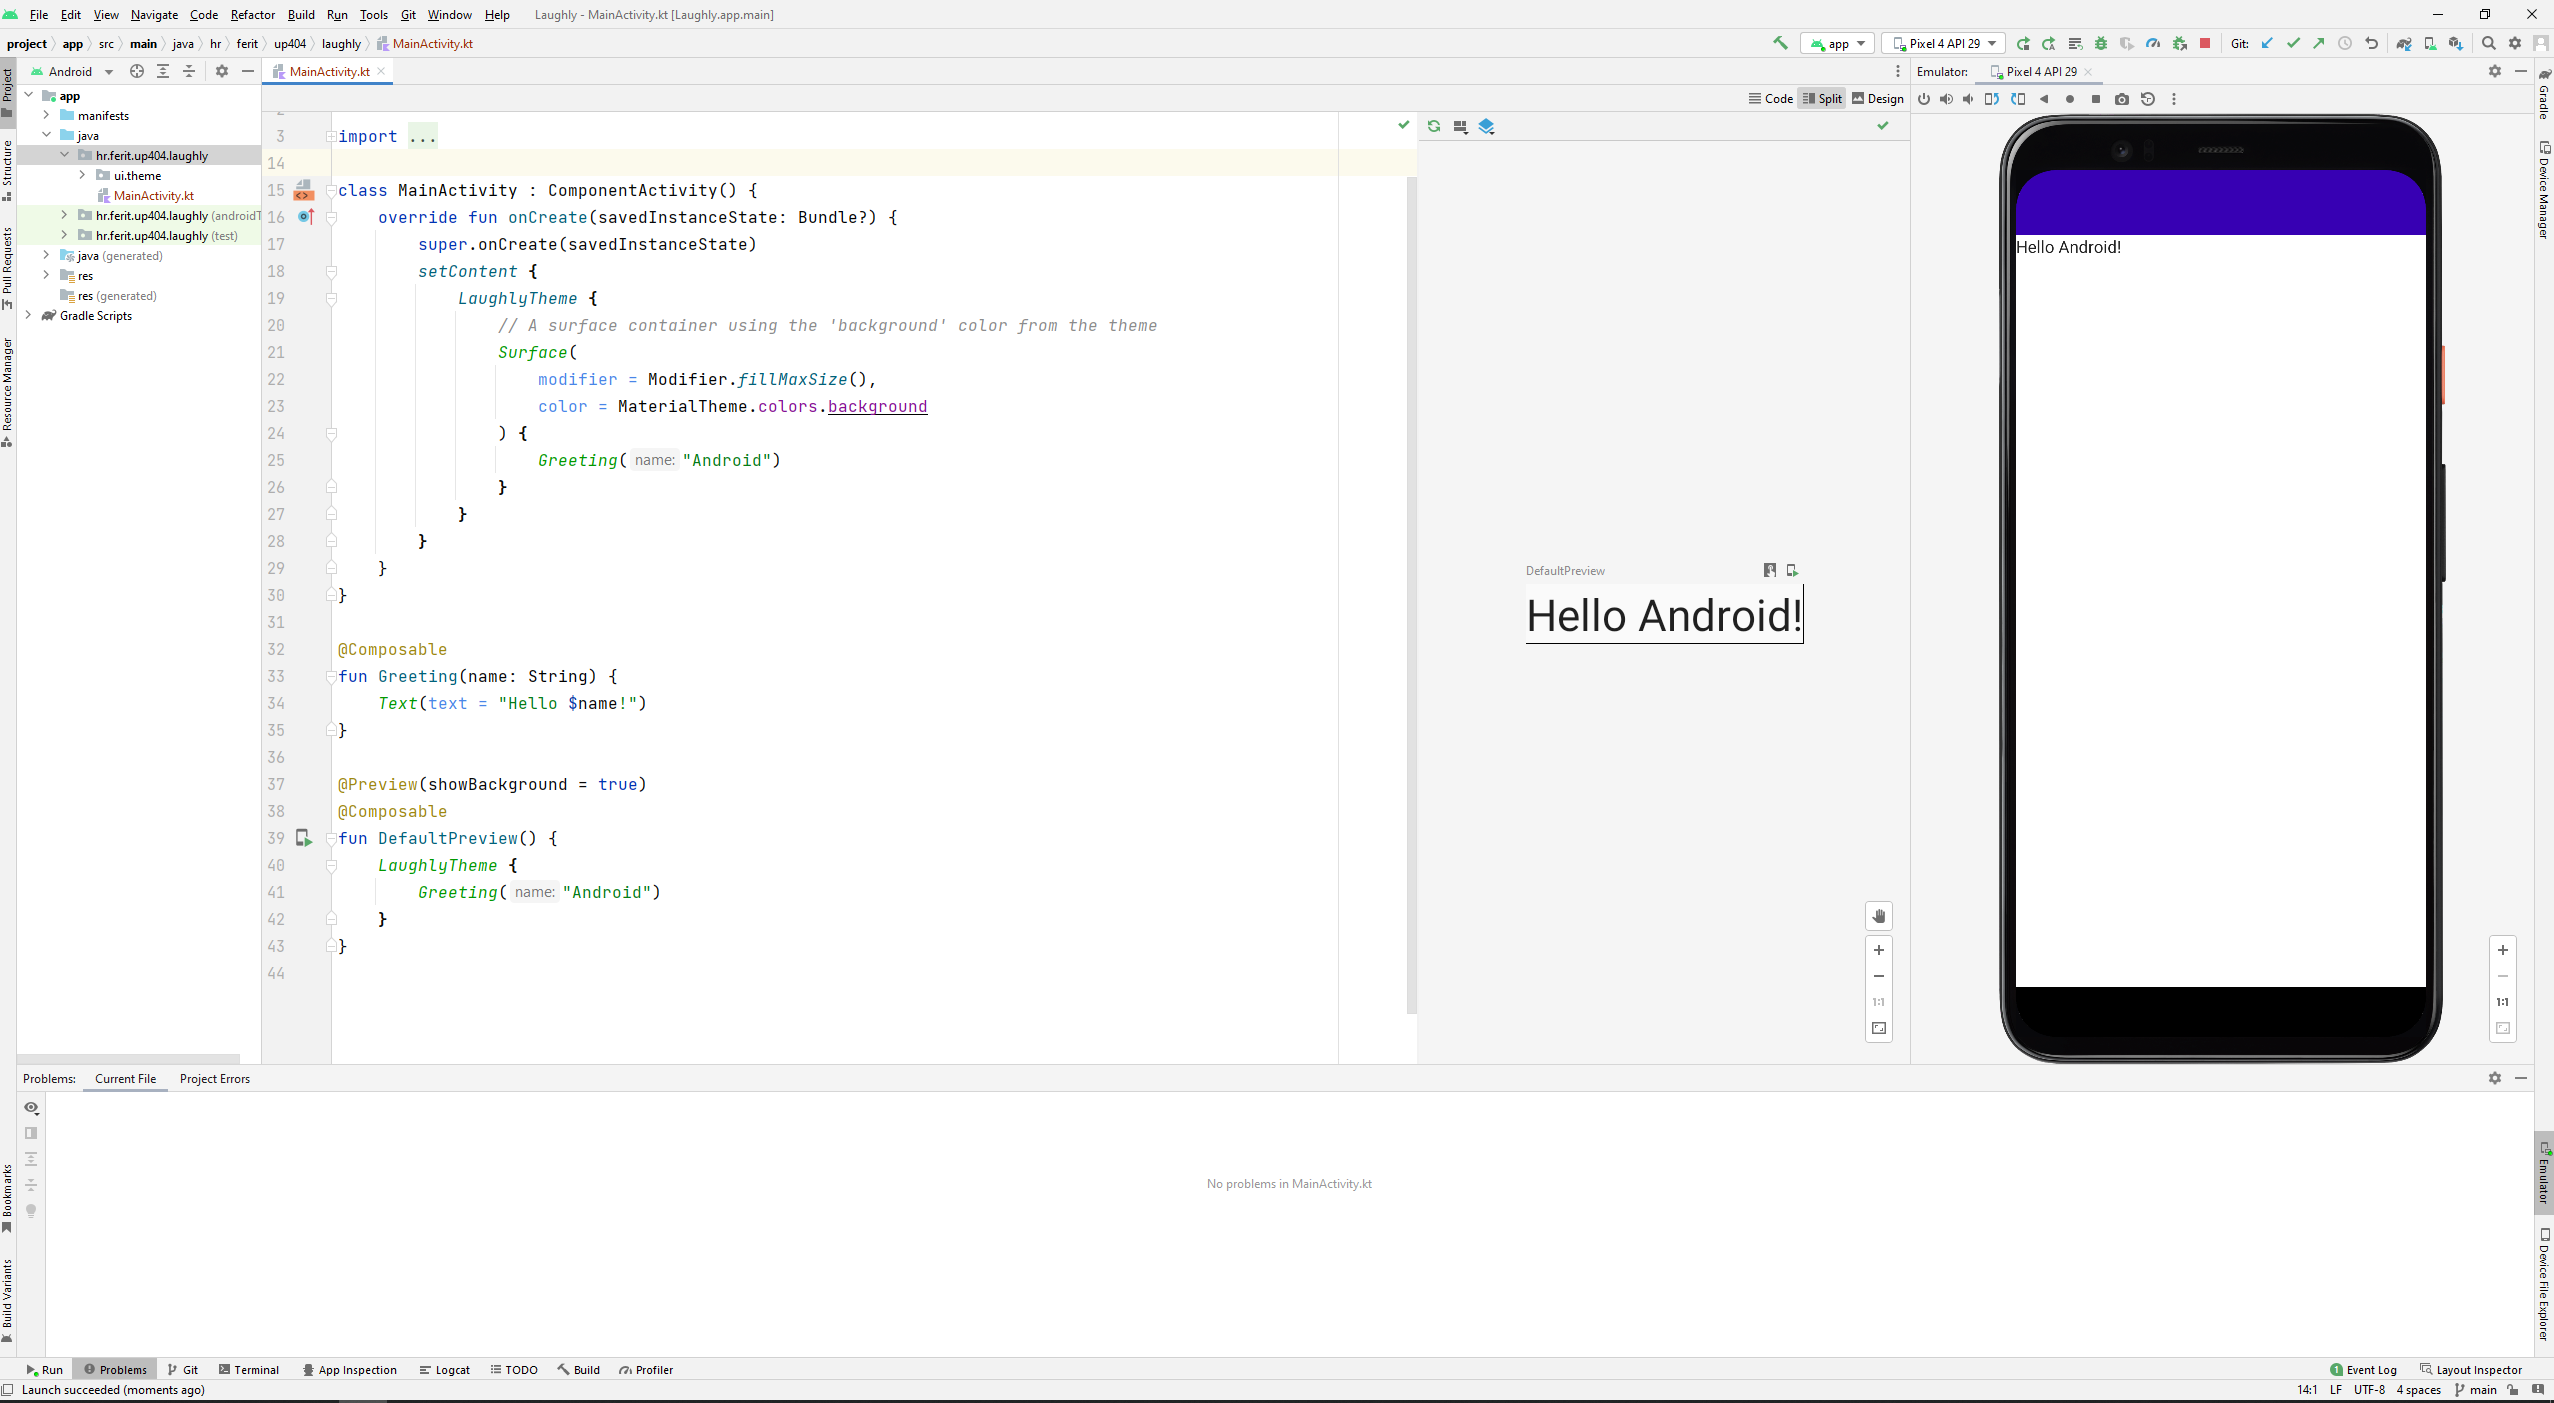
\includegraphics[width=\textwidth]{new_project_04.png}
	\caption{Kreiranje novog projekta - 4. korak}
	\label{fig:new_project_04}	
\end{figure}

\section{Uvođenje ekrana i navigacija}
\section{Značajka - inspiracija}
\section{Značajka - igra}
\section{Značajka - šala}
\section{Što dalje?}

	
	
	content...
	\begin{lstlisting}[caption={Simple code listing.}, label={lst:example1}, language=Kotlin]
		// this is a simple code listing:
		println("hello kotlin from latex")
	\end{lstlisting}
\end{document}